\documentclass{article}
\usepackage[margin=2.5cm, top=4cm, headheight=25pt]{geometry}
\usepackage{amsmath, amssymb, enumitem, fancyhdr, graphicx}
\usepackage[indent=20pt]{parskip}
\usepackage[hidelinks]{hyperref}
\usepackage{xcolor}
\usepackage{listings}
\usepackage{subcaption}
\usepackage{url}
\usepackage[most]{tcolorbox}
\usepackage{lastpage}
\usetikzlibrary{arrows, shapes}

\tcbuselibrary{listingsutf8} % Support for lstlistings within tcolorbox

\newtcolorbox[auto counter, number within=section]{question}[1][]{%
    colframe=gray!80,                      % Dark gray frame
    colback=gray!5,                       % Light gray background
    coltitle=black,                        % Black title
    title=\textbf{Question~\thetcbcounter}, % Bold title
    fonttitle=\bfseries\large,             % Subtle title font size
    rounded corners,                   % Slightly more rounded corners
    boxrule=0.25mm,                         % Thinner border for a sleek look
    enhanced,                              % Enhanced box features
    attach boxed title to top left={xshift=2mm, yshift=-2mm},
    boxed title style={colframe=gray!80, colback=gray!5, boxrule=0.25mm},
    % Title styling
    #1
}

\bibliographystyle{IEEEtran}
\graphicspath{{./images/}}

% -- Custom Variables --
\def\me{Rajdeep Gill 7934493}
\def\course{ECE 4260}
\def\labsection{A01}

\def\labno{4}
\def\title{Assignment \labno}

% -- Styling for code snippets --
\lstset{
    basicstyle=\ttfamily\scriptsize,           % Basic font style
    keywordstyle=\color{blue},            % Keywords color
    commentstyle=\color{gray},            % Comments color
    stringstyle=\color{teal},             % Strings color
    numbers=left,                         % Line numbers on the left
    numberstyle=\tiny\color{gray},        % Line number style
    stepnumber=1,                         % Line number step
    numbersep=10pt,                       % Space between line numbers and code
    backgroundcolor=\color{lightgray!10}, % Background color
    frame=single,                         % Adds a frame around the code
    breaklines=true,                      % Line breaking for long lines
    captionpos=b,                         % Caption position
    showspaces=false,                     % Don't show spaces
    showstringspaces=false                % Don't show spaces in strings
}
\renewcommand{\lstlistingname}{Code Snippet}

\renewcommand{\arraystretch}{1.2} % For less-ugly tables
\setlength\parindent{0pt}

%----- Samples 
% Questions:
%   \begin{question}[title=Custom Question Title]
%       Question details
%   \end{question}

% Tables:
%   \begin{table}[htbp]
%       \centering
%       \caption{Table Caption}
%       \begin{tabular}{ll}
%           \toprule
%           \textbf{Column 1} & \textbf{Column 2} \\
%           \midrule
%           Row 1 & Row 2 \\
%           Row 3 & Row 4 \\
%           \bottomrule
%       \end{tabular}
%   \end{table} 

% Figures:
%   Single figure:
%       \begin{figure}[htbp]
%           \centering
%           \includegraphics[width=0.5\textwidth]{example-image}
%           \caption{Figure Caption}
%       \end{figure}
%   Multiple figures:
%       \begin{figure}[htbp]
%           \centering
%           \begin{subfigure}[b]{0.5\textwidth}
%               \includegraphics[width=\textwidth]{example-image-a}
%               \caption{First subfigure}
%           \end{subfigure}
%           \begin{subfigure}[b]{0.5\textwidth}
%               \includegraphics[width=\textwidth]{example-image-b}
%               \caption{Second subfigure}
%           \end{subfigure}
%           \caption{Main figure}
%       \end{figure}

\begin{document}

% --------------------------------------------------------------------------------
% TITLE
% --------------------------------------------------------------------------------

\begin{center}
    \huge \title

    \vspace{2mm}
    \hrule

    \vspace{4mm}
    \large \me

    \vspace{2mm}
    \large \course~\labsection

    \vspace{2mm}
    \today
\end{center}

\vspace{4mm}

% --------------------------------------------------------------------------------
% END TITLE
% --------------------------------------------------------------------------------

\newpage


\vspace{1cm}
\newpage

\pagestyle{fancy}
\fancyhead[L]{\large Assignment \labno}
\fancyhead[R]{\large \me}

\fancyfoot[C]{Page \thepage~of~\pageref{LastPage}}

% --------------------------------------------------------------------------------
% BODY
% --------------------------------------------------------------------------------
\section{Problem 1}
\subsection{Part I}
\begin{enumerate}[label=1.\arabic*]
    \item Show the following is true:
    \begin{align*}
        \int_{0}^{T} g(x) \, dx = \int_{-T/2}^{T/2} g(x) \, dx
    \end{align*}

    Using the fact that $g(x) = g(x+T)$, we can write the integral as:
    \begin{align*}
        \int_{0}^{T} g(x) \, dx &= \int_{0}^{T/2} g(x) \, dx + \int_{T/2}^{T} g(x) \, dx \\
        &= \int_{0}^{T/2} g(x) \, dx + \int_{T/2}^{T} g(x-T) \, dx \\
        &= \int_{0}^{T/2} g(x) \, dx + \int_{-T/2}^{0} g(x) \, dx \\
        &= \int_{-T/2}^{T/2} g(x) \, dx
    \end{align*}

    \item We can deduce that $J_n(y)$ is also given by:
    \begin{align*}
        J_n(y) = \frac{1}{2\pi} \int_{-\pi}^{\pi} e^{j(y\sin(x)-nx)} \, dx = \frac{1}{2\pi} \int_{0}^{2\pi} e^{j(y\sin(x)-nx)} \, dx
    \end{align*}

    We can show this with the result from 1.1, as the function we are integrating over is $2\pi$ periodic. That is:
    \begin{align*}
        f(x, y) &= e^{j(y\sin(x)-nx)} \\
        f(x+2\pi, y) &= e^{j(y\sin(x+2\pi)-n(x+2\pi))} = e^{j(y\sin(x)-nx)} = f(x, y)
    \end{align*}

    Thus, the integral goes to:
    \begin{align*}
        J_n(y) &= \frac{1}{2\pi} \int_{-\pi}^{\pi} e^{j(y\sin(x)-nx)} \, dx \\
        &= \frac{1}{2\pi} \int_{-T/2}^{T/2} f(x, y) \, dx \\
        &= \frac{1}{2\pi} \int_{0}^{T} f(x, y) \, dx \\
        &= \frac{1}{2\pi} \int_{0}^{2\pi} e^{j(y\sin(x)-nx)} \, dx
    \end{align*}

    \item We can deduce from (6) the following:
    \begin{align*}
        J_{-n}(y) = (-1)^n J_n(y)
    \end{align*}

    We start with the definition of $J_{-n}(y)$:
    \begin{align*}
        J_{-n}(y) &= \frac{1}{2\pi} \int_{-\pi}^{\pi} e^{j(y\sin(x)+nx)} \, dx, \quad \text{Let } t = x + \pi \\
        &= \frac{1}{2\pi} \int_{0}^{2\pi} e^{j(y\sin(t-\pi)+n(t-\pi))} \, dt \\
        &= \frac{1}{2\pi} \int_{0}^{2\pi} e^{j(-y\sin(t)+nt)}e^{-j\pi n} \, dt \\
        &= \frac{(-1)^n}{2\pi} \int_{0}^{2\pi} e^{-j(y\sin(t)-nt)} \, dt, \quad \text{Let } u = -t + 2\pi \\
        &= \frac{(-1)^n}{2\pi}\int_{0}^{2\pi}e^{-j(y\sin(2\pi - u) - n(2\pi - u))} \, du \\
        &= \frac{(-1)^n}{2\pi}\int_{0}^{2\pi} e^{-j(-y\sin(u) +nu)}e^{jn2\pi} \, du \\
        &= \frac{(-1)^n}{2\pi}\int_{0}^{2\pi}e^{j(y\sin(u) - nu)} \, du = (-1)^n J_n(y)
    \end{align*}

    \item We can show that $J_n(y)$ is real-valued for all $y \in \mathbb{R}$:
    \begin{align*}
        J_n(y)^* &= \left( \frac{1}{2\pi} \int_{0}^{2\pi} e^{j(y\sin(x)-nx)} \, dx \right)^* \\
        &= \frac{1}{2\pi} \int_{0}^{2\pi} e^{-j(y\sin(x)-nx)} \, dx \\
        &= \frac{1}{2\pi} \int_{0}^{2\pi} e^{j(y\sin(-x)-n(-x))} \, dx, \quad \text{Let } u = -x + 2\pi \\
        &= \frac{1}{2\pi} \int_{0}^{2\pi} e^{j(y\sin(u+2\pi)-n(u+2\pi))} \, du \\ 
        &= \frac{1}{2\pi} \int_{0}^{2\pi} e^{j(y\sin(u)-nu)} \, du = J_n(y)
    \end{align*}
    Since the complex conjugate of $J_n(y)$ is equal to $J_n(y)$, $J_n(y)$ is real-valued for all $y \in \mathbb{R}$.

    \item We can find the deviation ratio as follows. We are given the equations for the frequency deviation, $\beta$
    \begin{align*}
        \beta &= \frac{\Delta f}{B} \\
        \text{Where } &\Delta f = \frac{k_f m_p}{2\pi}
    \end{align*}

    We have our message signal, $m(t)$ as:
    \begin{align*}
        m(t) = \alpha \cos(\omega_m t)
    \end{align*}

    Which has a maxmimum value of $\alpha$, and a bandwidth of $\omega_m / 2\pi$. We can find the deviation ratio, $\beta$ as:
    \begin{align*}
        \beta = \frac{\Delta f}{B} = \frac{k_f \alpha}{2\pi \frac{\omega_m}{2\pi}} = \frac{k_f \alpha}{\omega_m}
    \end{align*}

    \item We can show the FM-modulated signal corresponding to $m(t)$ is given by:
    \begin{align*}
        x_{FM}(t) = A \cos\left(\omega_c t + k_f a(t)\right)
    \end{align*}

    We assume initially that $a(-\infty) = 0$, and we can find $a(t)$ as:
    \begin{align*}
        a(t) &= \int_{-\infty}^{t} m(\tau) \, d\tau = \int_{-\infty}^{t} \alpha \cos(\omega_m \tau) \, d\tau \\
        &= \frac{\alpha}{\omega_m} \sin(\omega_m t)
    \end{align*}

    We also recognize that:
    \begin{align*}
        k_f a(t) = \frac{\alpha k_f}{\omega_m} \sin(\omega_m t) = \beta \sin(\omega_m t)
    \end{align*}

    Thus, we have:
    \begin{align*}
        x_{FM}(t) = A\cos\left(\omega_c t + \beta\sin(\omega_m t)\right)
    \end{align*}

    We know that $\cos(\theta)$ is the real part of $e^{j\theta}$, and we can write the FM-modulated signal as:
    \begin{align*}
        x_{FM}(t) &= \mathfrak{R} \left\{Ae^{j\left(\omega_c t + \beta\sin(\omega_m t)\right)}\right\} \\
        &= A \, \mathfrak{R}\left\{e^{j\omega_c t}e^{j\beta\sin(\omega_m t)}\right\} \\
        &= A \, \mathfrak{R}\left\{e^{j\omega_c t} z(t)\right\}
    \end{align*}

    Where $z(t) = e^{j\beta\sin(\omega_m t)}$.

    \item We can show that the signal $z(t)$ is periodic with period $T = 2\pi/\omega_m$:
    \begin{align*}
        z(t+2\pi/\omega_m) &= e^{j\beta\sin(\omega_m (t+2\pi/\omega_m))} \\
        &= e^{j\beta\sin(\omega_m t + 2\pi)} \\
        &= e^{j\beta\sin(\omega_m t)} \\
        &= z(t)
    \end{align*}

    Thus, $z(t)$ is periodic with period $T = 2\pi/\omega_m$.

    \item We can show the relationship between the fourier series coefficients of $z(t)$ and $J_n(\beta)$ as follows. We start with the definition of the fourier series coefficients of $z(t)$:
    \begin{align*}
        z_n &= \frac{\omega_m}{2\pi} \int_{\pi/\omega_m}^{\pi/\omega_m} z(t) e^{-jn\omega_m t} \, dt \\
        &= \frac{\omega_m}{2\pi} \int_{-\pi/\omega_m}^{\pi/\omega_m} e^{j\beta\sin(\omega_m t)} e^{-jn\omega_m t} \, dt \\
        &= \frac{\omega_m}{2\pi} \int_{-\pi/\omega_m}^{\pi/\omega_m} e^{j(\beta\sin(\omega_m t) - n\omega_m t)} \, dt, \quad \text{Let } x = \omega_m t \\
        &= \frac{1}{2\pi} \int_{-\pi}^{\pi} e^{j(\beta\sin(x) - nx)} \, dx = J_n(\beta)
    \end{align*}

    \item We can show the FM-modulated signal $x_{FM}(t)$ can be written as:
    \begin{align*}
        x_{FM}(t) = A \sum_{n=-\infty}^{\infty} J_n(\beta) \cos\left(2\pi\left[f_c+nf_m\right]t\right)
    \end{align*}

    Using the results from 1.6 and 1.7, we have:
    \begin{align*}
        x_{FM}(t) &= A \, \mathfrak{R}\left\{e^{j\omega_c t} z(t)\right\} \\
        &= A \, \mathfrak{R}\left\{e^{j\omega_c t} \sum_{n=-\infty}^{\infty} z_n e^{jn\omega_m t}\right\} \\
        &= A \, \mathfrak{R}\left\{\sum_{n=-\infty}^{\infty} z_n e^{j(\omega_c + n\omega_m)t}\right\} \\
        &= A \sum_{n=-\infty}^{\infty} J_n(\beta) \cos\left(\omega_ct + n\omega_mt\right) \\
        &= A \sum_{n=-\infty}^{\infty} J_n(\beta) \cos\left(2\pi\left[f_c+nf_m\right]t\right)
    \end{align*}

    \item Plugging in the provided values into $x_{FM}(t)$, we have:
    \begin{align*}
        \beta = \frac{k_f \alpha}{\omega_m} = \frac{2\pi \times 10^5 \cdot 6}{2\pi \times 300 \times 10^3} = 2 \\
        x_{FM}(t) = 2\sum_{n=-\infty}^{\infty} J_n(2) \cos\left(2\pi\left[f_c + n\cdot 300 \times 10^3\right]t\right)
    \end{align*}

    The fourier transform of $x_{FM}(t)$ is given by:
    \begin{align*}
        X_{FM}(f) = \sum_{n=-\infty}^{\infty} J_n(2) \left(
            \delta(f - (f_c + n\cdot 300 \times 10^3)) + \delta(f + (f_c + n\cdot 300 \times 10^3))
        \right)
    \end{align*}

    Assuming that $J_n(2)$ is negligible for $n > 3$, we can plot from $n = -3$ to $n = 3$. We will also utilize the fact that $J_{-n}(y) = (-1)^n J_n(y)$.
    \begin{align*}
        n &= -3: \quad -J_{3}(2)\left(\delta(f + (f_c - 900 \times 10^3)) + \delta(f - (f_c - 900 \times 10^3))\right) \\
        n &= -2: \quad J_{2}(2)\left(\delta(f + (f_c - 600 \times 10^3 )) + \delta(f - (f_c + 600 \times 10^3))\right) \\
        n &= -1: \quad -J_{1}(2)\left(\delta(f + (f_c - 300 \times 10^3 )) + \delta(f - (f_c - 300 \times 10^3))\right) \\
        n &= 0: \quad J_{0}(2)\left(\delta(f + f_c) + \delta(f - f_c)\right) \\
        n &= 1: \quad J_{1}(2)\left(\delta(f + (f_c + 300 \times 10^3 )) + \delta(f - (f_c + 300 \times 10^3))\right) \\
        n &= 2: \quad J_{2}(2)\left(\delta(f + (f_c + 600 \times 10^3 )) + \delta(f - (f_c + 600 \times 10^3))\right) \\
        n &= 3: \quad J_{3}(2)\left(\delta(f + (f_c + 900 \times 10^3 )) + \delta(f - (f_c + 900 \times 10^3))\right)
    \end{align*}
    \newpage
    Plotting the magnitude, $|X_{FM}(f)|$, we get the following result seen in \autoref{fig:p1_10}.
    \begin{figure}[ht!]
        \centering
        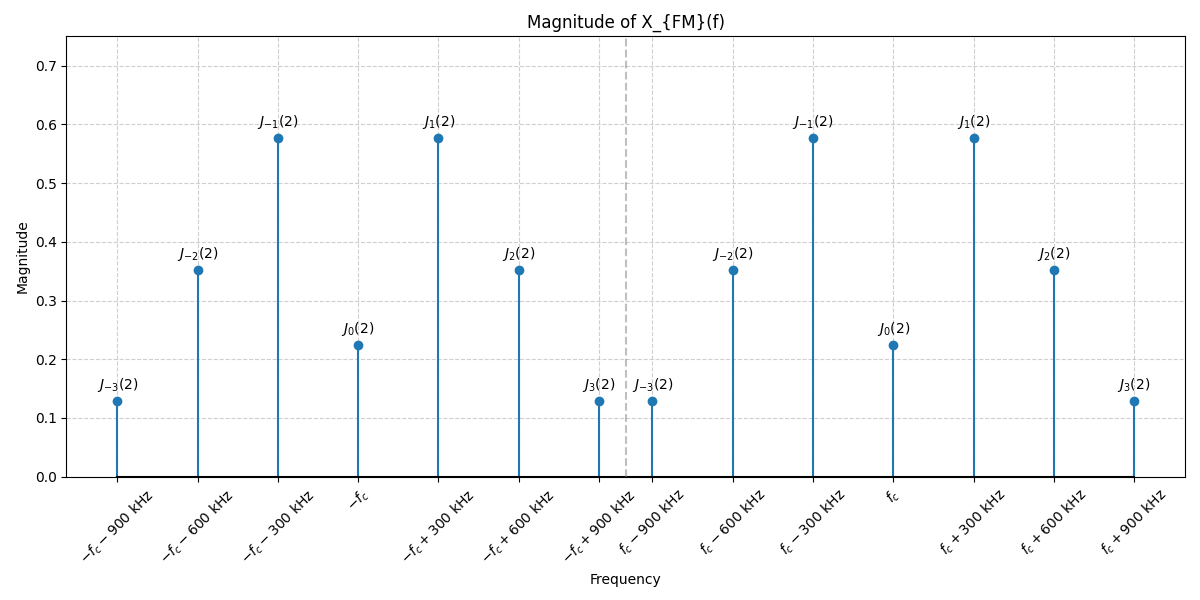
\includegraphics[width=0.8\textwidth]{X_FM.png}
        \caption{Fourier Transform of $x_{FM}(t)$}
        \label{fig:p1_10}
    \end{figure}


\end{enumerate}


\newpage
\newpage
\section{Problem 2}

\begin{enumerate}[label=2.\arabic*]
    \item Determine and sketch $G_+(f)$

    Since $g_+(t)$ is defined as:
    \[
        g_+(t) = g(t) + j\hat{g}(t), \quad \text{where } \hat{g}(t) = \frac{1}{\pi t} \ast g(t)
    \]

    The fourier transform of $g_+(t)$ is given by:
    \begin{align*}
        \mathcal{F}\{g_+(t)\} &= \mathcal{F}\{g(t)\} + j\mathcal{F}\{\hat{g}(t)\} \\
        &= G(f) + jG(f)H(f)
\end{align*}

Where $H(f)$ is the fourier transform of $\frac{1}{\pi t}$, which is given by:
\begin{align*}
    H(f) = \frac{1}{j} \text{sgn}(f) = \begin{cases}
        -j & f > 0 \\
        j & f < 0
    \end{cases}
\end{align*}

Therefore we have:
\begin{align*}
        G_+(f) &= G(f) + jG(f)H(f) = G(f) + \text{sgn}(f)G(f) \\
        &= \begin{cases}
            2G(f) & f > 0 \\
            0 & f < 0
        \end{cases}
\end{align*}

The plot of $G_+(f)$ can be seen in \autoref{fig:p2_1}.
\begin{figure}[ht!]
    \centering
    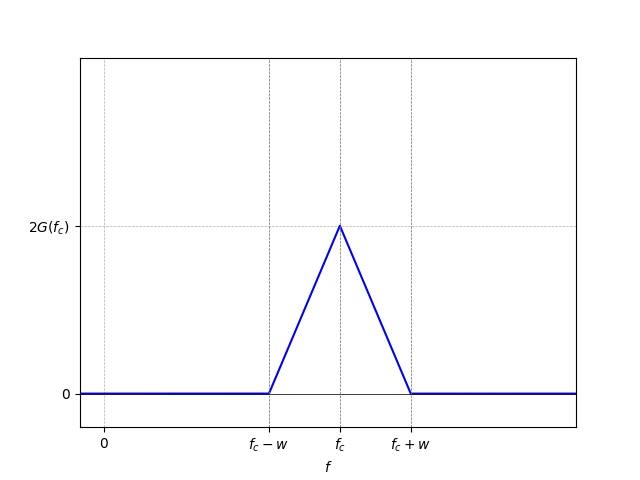
\includegraphics[width=0.5\textwidth]{p2_1.png}
    \caption{Plot of $G_+(f)$}
    \label{fig:p2_1}
\end{figure}

\item Given that $\tilde{g}(t) = g_+(t)e^{-j2\pi f_c t}$, the fourier transform of $\tilde{g}(t)$ is given by:
\begin{align*}
        \text{Using: } \mathcal{F}\{g(t)e^{j2\pi f_0 t}\} = G(f-f_0) \\
        \mathcal{F}\{\tilde{g}(t)\} = G_+(f+f_c)
\end{align*}

The plot of $\tilde{G}(f)$ can be seen in \autoref{fig:p2_2}. It is just a shifted version of $G_+(f)$, with the triangular pulse centered at $f = 0$.
\begin{figure}
    \centering
    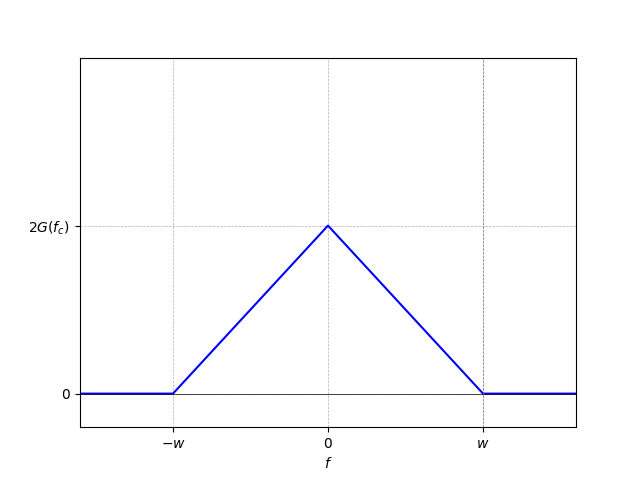
\includegraphics[width=0.5\textwidth]{p2_2.png}
    \caption{Plot of $\tilde{G}(f)$}
    \label{fig:p2_2}
\end{figure}

\item We can show that:
\begin{align*}
    g(t) = \mathfrak{R}\left\{\tilde{g}(t)e^{j2\pi f_c t}\right\} 
\end{align*}

We expand the right side of the equation:
\begin{align*}
    \mathfrak{R}\left\{\tilde{g}(t)e^{j2\pi f_c t}\right\} &= \mathfrak{R}\left\{g_+(t)e^{-j2\pi f_c t}e^{j2\pi f_c t}\right\} \\
    &= \mathfrak{R}\left\{g_+(t)\right\} \\
    &= \mathfrak{R}\left\{g(t) + j\hat{g}(t)\right\} = g(t)
\end{align*}

    Thus, we have shown that $g(t) = \mathfrak{R}\left\{\tilde{g}(t)e^{j2\pi f_c t}\right\}$.

    \item We can find the complex envelopes $\tilde{v}(t), \tilde{h}(t)$ as follows.
    
    Using the result from 2.3 we can write $v(t)$ and find the envelope $\tilde{v}(t)$:
    \begin{align*}
        v(t) &= g(t)s(t) = \mathfrak{R}\left\{g(t)\left(e^{j(2\pi f_c t - \pi k t^2)}\right)\right\} = \mathfrak{R} \left\{g(t)e^{j2\pi f_c t}e^{-j\pi k t^2}\right\} = \mathfrak{R}\left\{\tilde{v}(t)e^{j2\pi f_c t}\right\} \\
        &\implies \tilde{v}(t) = g(t)e^{-j\pi k t^2}
    \end{align*}

    Similarily for $h(t)$:
    \begin{align*}
        h(t) &= \cos(2\pi f_c t + \pi k t^2) = \mathfrak{R}\left\{e^{j(2\pi f_c t + \pi k t^2)}\right\} = \mathfrak{R}\left\{e^{j2\pi f_c t}e^{j\pi kt^2}\right\} = \mathfrak{R}\left\{\tilde{h}(t)e^{j2\pi f_c t}\right\} \\
        &\implies \tilde{h}(t) = e^{j\pi k t^2}
    \end{align*}

    \item We can find the complex envelope $\tilde{z}(t)$ as follows:
    \begin{align*}
        \tilde{z}(t) = \tilde{v}(t) \ast \tilde{h}(t) &= g(t)e^{-j\pi k t^2} \ast e^{j\pi k t^2} \\
        &= \int_{-\infty}^{\infty} g(\tau)e^{-j\pi k \tau^2}e^{j\pi k (t-\tau)^2} \, d\tau \\
        &= \int_{-\infty}^{\infty} g(\tau)e^{-j\pi k \tau^2}e^{j\pi k t^2}e^{-j2\pi k t\tau}e^{j\pi k \tau^2} \, d\tau \\
        &= e^{j\pi k t^2} \int_{-\infty}^{\infty} g(\tau)e^{-j2\pi (k t)\tau} \, d\tau \\
        &= e^{j\pi k t^2} G(kt)
    \end{align*}

\end{enumerate}


\section{Problem 3}

\begin{enumerate}[label=3.\arabic*]
    \item We can show the relationship between the fourier coefficents of $g(t)$ and $\dot{g}(t)$ as follows. The relationship is given by:
    \begin{align*}
        \dot{g}_n = jn\omega_0 g_n
    \end{align*}
    We start with the definition of $\dot{g}(t)$:
    \begin{align*}
        \dot{g}(t) = \frac{d}{dt} g(t) &= \frac{d}{dt} \sum_{n=-\infty}^{\infty} g_n e^{jn\omega_0 t} \\
        &= \sum_{n=-\infty}^{\infty} jn\omega_0 g_n e^{jn\omega_0 t} = \sum_{n=-\infty}^{\infty} \dot{g}_n e^{jn\omega_0 t} \\
        \implies jn\omega_0 g_n &= \dot{g}_n
    \end{align*}

    \item Given that $m(t)$ are triangular pulses, with the time period of $2\times10^{-4}$ seconds, the derivative, $\dot{m}(t)$, will be square pulses, with the same time period. We can find the fourier coefficents of $\dot{m}(t)$ and then relate them to the fourier coefficents of $m(t)$ using the relationship from 3.1.
    
    We have that $m(t)$ is given by:
    \begin{align*}
        m(t) &= \begin{cases}
            2\cdot10^4t + 1 & -10^{-4} \leq t < 0 \\
            -2\cdot10^4t + 1 & 0 \leq t < 10^{-4} \\
        \end{cases} \\
        m(t) &= m(t+2\times10^{-4})
    \end{align*}

    Therefore, we can find $\dot{m}(t)$ as:
    \begin{align*}
        \dot{m}(t) &= \begin{cases}
            2\cdot10^4 & -10^{-4} \leq t < 0 \\
            -2\cdot10^4 & 0 \leq t < 10^{-4} \\
        \end{cases} \\
        \dot{m}(t) &= \dot{m}(t+2\times10^{-4})
    \end{align*}

    The fourier series of $\dot{m}(t)$ is given by:
    \begin{align*}
        \dot{m}_n &= \frac{1}{T} \int_{T} \dot{m}(t) e^{-j2\pi \frac{n}{T} t} \, dt \\
        &= \frac{1}{2\times10^{-4}} \int_{-10^{-4}}^{10^{-4}} \dot{m}(t) e^{-j2\pi \frac{n}{2\times10^{-4}} t} \, dt \\
        &= \frac{1}{2\times 10^{-4}} \int_{-10^{-4}}^{0} 2\cdot10^4 e^{-j\pi n10^{4} t} \, dt + \frac{1}{2\times 10^{-4}} \int_{0}^{10^{-4}} -2\cdot10^4 e^{-j\pi n10^{4}t} \, dt \\
    \end{align*}

    The first integral evaluates to:
    \begin{align*}
        2\times10^4\int_{-10^{-4}}^{0} e^{-j\pi n10^{4}t} \, dt &= \frac{2\times10^4}{-j\pi n10^{4}}\left(e^{-j\pi n10^{4}t}\right)\Big|_{-10^{-4}}^{0} \\
        &= \frac{-2}{j\pi n}\left(1 - e^{j\pi n}\right) \\
        &= \frac{2\cdot(-1)^n - 2}{j\pi n}
    \end{align*}

    The second integral evaluates to:
    \begin{align*}
        -2\times10^4\int_{0}^{10^{-4}} e^{-j\pi n10^{4}t} \, dt &= \frac{-2\times10^4}{-j\pi n10^{4}}\left(e^{-j\pi n10^{4}t}\right)\Big|_{0}^{10^{-4}} \\
        &= \frac{2}{j\pi n}\left(e^{-j\pi n} - 1\right) \\
        &= \frac{2\cdot(-1)^n - 2}{j\pi n}
    \end{align*}

    Putting it all together, we have:
    \begin{align*}
        \dot{m}_n &= \frac{1}{2\times10^{-4}}\left(\frac{2\cdot(-1)^n - 2}{j\pi n} + \frac{2\cdot(-1)^n - 2}{j\pi n}\right) = \frac{4\cdot(-1)^n - 4}{j\pi n} \cdot \frac{1}{2\times10^{-4}} \\
        &= \frac{2\cdot(-1)^n - 2}{j\pi n} \cdot 10^4
    \end{align*}

    Using the relationship from 3.1, we have:
    \begin{align*}
        m_n = \frac{\dot{m}_n}{jn\omega_0}, \quad \text{Where } \omega_0 = \frac{2\pi}{T} = \frac{2\pi}{2\times10^{-4}} = 10^4\pi \\
        m_n = \frac{1}{jn\omega_0} \cdot \frac{2\cdot(-1)^n - 2}{j\pi n} \cdot 10^4 = \frac{2-2\cdot(-1)^n}{\pi^2 n^2} \\
        m_n = \begin{cases}
            \frac{4}{\pi^2 n^2} & n \text{ odd} \\
            0 & n \text{ even}
        \end{cases}
    \end{align*}

    For $n=0$, we have:
    \begin{align*}
        \dot{m}_0 = \frac{1}{2\times10^{-4}}\int_{-10^{-4}}^{10^{-4}} \dot{m}(t) \, dt = 0
    \end{align*}
    This is $\dot{m}(t)$ is an odd function, and the integral of an odd function over a symmetric interval is 0.

    \item We can find the power, $P_m$, of $m(t)$ using integration as follows:
    \begin{align*}
        P_m = \frac{1}{T} \int_{T} |m(t)|^2 \, dt = \frac{1}{2\times10^{-4}} \left(
            \int_{-10^{-4}}^{0} (2\cdot10^4t + 1)^2 \, dt + \int_{0}^{10^{-4}} (-2\cdot10^4t + 1)^2 \, dt
        \right)
    \end{align*}

    The first integral evaluates to:
    \begin{align*}
        \frac{1}{2\times 10^{-4}}\int_{-10^{-4}}^{0} (2\cdot10^4t + 1)^2 \, dt &= \frac{1}{2\times10^{-4}} \int_{-10^{-4}}^{0} (4\cdot10^8t^2 + 4\cdot10^4t + 1) \, dt \\
        &= \frac{1}{2\times10^{-4}} \left(\frac{4\cdot10^8}{3}t^3 + 2\cdot10^4t^2 + t\right)\Big|_{-10^{-4}}^{0} \\
        &= \frac{1}{2\times10^{-4}} \left(\frac{4\cdot10^8}{3}10^{-12} - 2\cdot10^4\cdot10^{-8} + 10^{-4}\right) \\
        &= \frac{1}{2\times10^{-4}} \left(\frac{4}{3} - 2 + 1 \right) \times 10^{-4} \\
        &= \frac{1}{6}
    \end{align*}

    Similarily, the second integral evaluates to:
    \begin{align*}
        \frac{1}{2\times 10^{-4}}\int_{0}^{10^{-4}} (-2\cdot10^4t + 1)^2 \, dt &= \frac{1}{2\times10^{-4}} \int_{0}^{10^{-4}} (4\cdot10^8t^2 - 4\cdot10^4t + 1) \, dt \\
        &= \frac{1}{2\times10^{-4}} \left(\frac{4\cdot10^8}{3}t^3 - 2\cdot10^4t^2 + t\right)\Big|_{0}^{10^{-4}} \\
        &= \frac{1}{2\times10^{-4}} \left(\frac{4\cdot10^8}{3}10^{-12} - 2\cdot10^4\cdot10^{-8} + 10^{-4}\right) \\
        &= \frac{1}{2\times10^{-4}} \left(\frac{4}{3} - 2 + 1 \right) \times 10^{-4} \\
        &= \frac{1}{6}
    \end{align*}

    Therefore we have:
    \begin{align*}
        P_m = \frac{1}{6} + \frac{1}{6} = \frac{1}{3}
    \end{align*}

    \item Using Parseval's theorem, we can find the power of $m(t)$ using the fourier coefficients as follows:
    \begin{align*}
        P_m = \sum_{n=-\infty}^{\infty} |m_n|^2 = \sum_{\substack{n=-\infty \\ n \text{ odd}}}^{\infty} \left|\frac{4}{\pi^2 n^2}\right|^2 &= \sum_{\substack{n=-\infty \\ n \text{ odd}}}^{\infty} \frac{16}{\pi^4 n^4} \\
        &= 2\times\left(\frac{16}{\pi^4}
            \sum_{n=0}^{\infty} \frac{1}{(2n+1)^4}
        \right) \\
        &= \frac{32}{\pi^4} \times \frac{\pi^4}{96} \\
        &= \frac{1}{3}
    \end{align*}

    \item We first find the bandwidth associated with the frequency-modulated signal $x_{FM}(t)$. We have that the instantaneous frequency deviation is:
    \begin{align*}
        f_i(t) = f_c + \frac{k_f}{2\pi}m(t)
    \end{align*}

    From this, we can find the min and max, $f_{\text{min}}, f_{\text{max}}$:
    \begin{align*}
        f_{\text{min}} = f_c + \frac{2\pi \times 10^5}{2\pi} \cdot (-1) = f_c - 10^5 \\
        f_{\text{max}} = f_c + \frac{2\pi \times 10^5}{2\pi} \cdot (1) = f_c + 10^5 \\
        B_{\text{FM}} = f_{\text{max}} - f_{\text{min}} = 2\times10^5 = 200 \text{ kHz}
    \end{align*}

    Similarily, we can find the bandwidth associated with the phase-modulated signal $x_{PM}(t)$. We have that the instantaneous phase deviation is:
    \begin{align*}
        f_i(t) = f_c + \frac{k_p}{2\pi}\dot{m}(t)
    \end{align*}

    From this, we can find the min and max, $f_{\text{min}}, f_{\text{max}}$:
    \begin{align*}
        f_{\text{min}} = f_c + \frac{5\pi}{2\pi} \cdot (-2\times10^4) = f_c - 5 \times 10^4 \\
        f_{\text{max}} = f_c + \frac{5\pi}{2\pi} \cdot (2\times10^4) = f_c + 5 \times 10^4 \\
        B_{\text{PM}} = f_{\text{max}} - f_{\text{min}} = 10^5 = 100 \text{ kHz}
    \end{align*}

    \item If we double the amplitude of the message signal, the bandwidth of the frequency-modulated signal and phase-modulated signal will also double. Let $m'(t) = 2m(t)$, then we have:
    \begin{align*}
        f_{\text{min}} = f_c + \frac{2\pi \times 10^5}{2\pi} \cdot (-2) = f_c - 2 \times 10^5 \\
        f_{\text{max}} = f_c + \frac{2\pi \times 10^5}{2\pi} \cdot (2) = f_c + 2 \times 10^5 \\
        B'_{\text{FM}} = f_{\text{max}} - f_{\text{min}} = 4\times10^5 = 400 \text{ kHz} = 2 \times 200 \text{ kHz} = 2B_{\text{FM}}
    \end{align*}
    Similarily for the phase-modulated signal:
    \begin{align*}
        f_{\text{min}} = f_c + \frac{5\pi}{2\pi} \cdot (-4\times10^4) = f_c - 10^5 \\
        f_{\text{max}} = f_c + \frac{5\pi}{2\pi} \cdot (4\times10^4) = f_c + 10^5 \\
        B'_{\text{PM}} = f_{\text{max}} - f_{\text{min}} = 2\times10^5 = 200 \text{ kHz} = 2 \times 100 \text{ kHz} = 2B_{\text{PM}}
    \end{align*}
\end{enumerate}


% --------------------------------------------------------------------------------
% END BODY
% --------------------------------------------------------------------------------

\end{document}
